% Point avec Mehdi, 20 juillet 2026. Version vulgarisee des slides tuteur (formules retirees).
% Compile avec Tectonic (pdfLaTeX standard). Figures partagees avec le point tuteur du 17/07.
% Objectif : presenter le modele cascade + contagion en clair, et recueillir l'avis operationnel
%            de Mehdi (data pour calibrer la contagion, maille de severite par pilier).
\documentclass[11pt]{beamer}
\usetheme{Madrid}
\usecolortheme{seahorse}
\usepackage[utf8]{inputenc}
\usepackage[T1]{fontenc}
\usepackage[french]{babel}
\usepackage{booktabs}
\graphicspath{{../cascade_qualitative/figures/}}
\setbeamertemplate{navigation symbols}{}
\setbeamertemplate{caption}{\raggedright\insertcaption\par}
\setbeamerfont{block title}{size=\small}

\title[Point Mehdi]{Mémoire SCR DORA : le modèle en clair}
\subtitle{Cascades entre piliers et contagion, sans le formalisme}
\author[K. Kaddouri]{Kélian Kaddouri}
\institute[ENSAE / Nexialog]{ENSAE / Nexialog Consulting}
\date[20/07/2026]{20 juillet 2026}

\begin{document}

\begin{frame}
\titlepage
\end{frame}

% =====================================================================
\begin{frame}{Pourquoi cet échange}
\begin{itemize}
\item Le mémoire relie trois choses : le risque \textbf{cyber}, la conformité \textbf{DORA}
      et le \textbf{capital de solvabilité} (SCR).
\item Point de départ : la Formule Standard sous-estime le cyber, parce qu'elle ne voit pas
      la \textbf{contagion} entre les fonctions d'une entité.
\item Je te présente le modèle en clair, sans les équations.
\end{itemize}
\vfill
\textbf{Ce que j'attends de toi :} ton regard opérationnel, et surtout un point de blocage
sur les \textbf{données} pour calibrer la contagion.
\end{frame}

% =====================================================================
\begin{frame}{L'idée centrale, en une phrase}
\begin{block}{}
On ne note pas un \textbf{ensemble} de piliers DORA touchés, mais une \textbf{chaîne
ordonnée} d'effondrement.
\end{block}
\begin{itemize}
\item Une cascade qui suit une direction causale plausible (la gouvernance qui lâche, puis
      les conséquences) est un vrai emballement : plus \textbf{probable} \emph{et} plus
      \textbf{grave}.
\item Le même ensemble de piliers pris \textbf{à l'envers} est rare et peu grave.
\end{itemize}
\vfill
\begin{center}
\textbf{C'est l'ordre qui pilote le verdict}, pas seulement la liste des piliers touchés.
\end{center}
\end{frame}

% =====================================================================
\begin{frame}{Les cinq piliers de DORA}
\begin{itemize}
\item \textbf{P1} : gouvernance et gestion du risque TIC (la fondation).
\item \textbf{P2} : gestion des incidents.
\item \textbf{P3} : tests de résilience (TLPT).
\item \textbf{P4} : gestion du risque lié aux tiers (cloud, prestataires critiques).
\item \textbf{P5} : partage d'informations (volontaire).
\end{itemize}
\vfill
Intuition de terrain : \textbf{P1 et P4} sont plutôt des déclencheurs en amont,
\textbf{P5} est plutôt en bout de chaîne.
\end{frame}

% =====================================================================
\begin{frame}{Trois jugements d'expert, rien d'autre}
Tout le modèle qualitatif tient sur trois barèmes, ordonnés à dire d'expert :
\begin{itemize}
\item \textbf{Qui amorce} : quel pilier a le plus de chances de démarrer une cascade.
\item \textbf{Qui entraîne qui} : la force du lien \og{}tel pilier en entraîne tel autre\fg{},
      et surtout elle est \textbf{asymétrique} (P1 entraîne beaucoup, l'inverse très peu).
\item \textbf{La gravité propre} de chaque pilier s'il tombe seul.
\end{itemize}
\vfill
\begin{block}{}
Tu reconnaîtras l'esprit du \textbf{RPN de l'AMDEC} et des matrices de criticité des
\textbf{dashboards ORSA}. La seule nouveauté : ici, la \textbf{direction} (qui entraîne qui)
change la note.
\end{block}
\end{frame}

% =====================================================================
\begin{frame}{La criticité : proba croisée avec gravité}
Comme une matrice de risque : criticité $=$ probabilité \textbf{croisée avec} gravité,
lue en catégories (de Faible à Extrême). Même paire de piliers, deux sens :
\begin{center}\small
\renewcommand{\arraystretch}{1.25}
\begin{tabular}{@{}lcc@{}}
\toprule
 & \textbf{1 vers 2} & \textbf{2 vers 1} \\
 & \emph{gouvernance puis incident} & \emph{incident puis gouvernance} \\
\midrule
Probabilité & Probable  & Très rare \\
Gravité     & Critique  & Modérée \\
\textbf{Criticité} & \textbf{Majeure} & \textbf{Faible} \\
\bottomrule
\end{tabular}
\end{center}
\vfill
Mêmes deux piliers, \textbf{verdict opposé} : tout l'écart vient de la cohérence causale de
l'ordre.
\end{frame}

% =====================================================================
\begin{frame}{L'ordre renverse le verdict}
\begin{center}
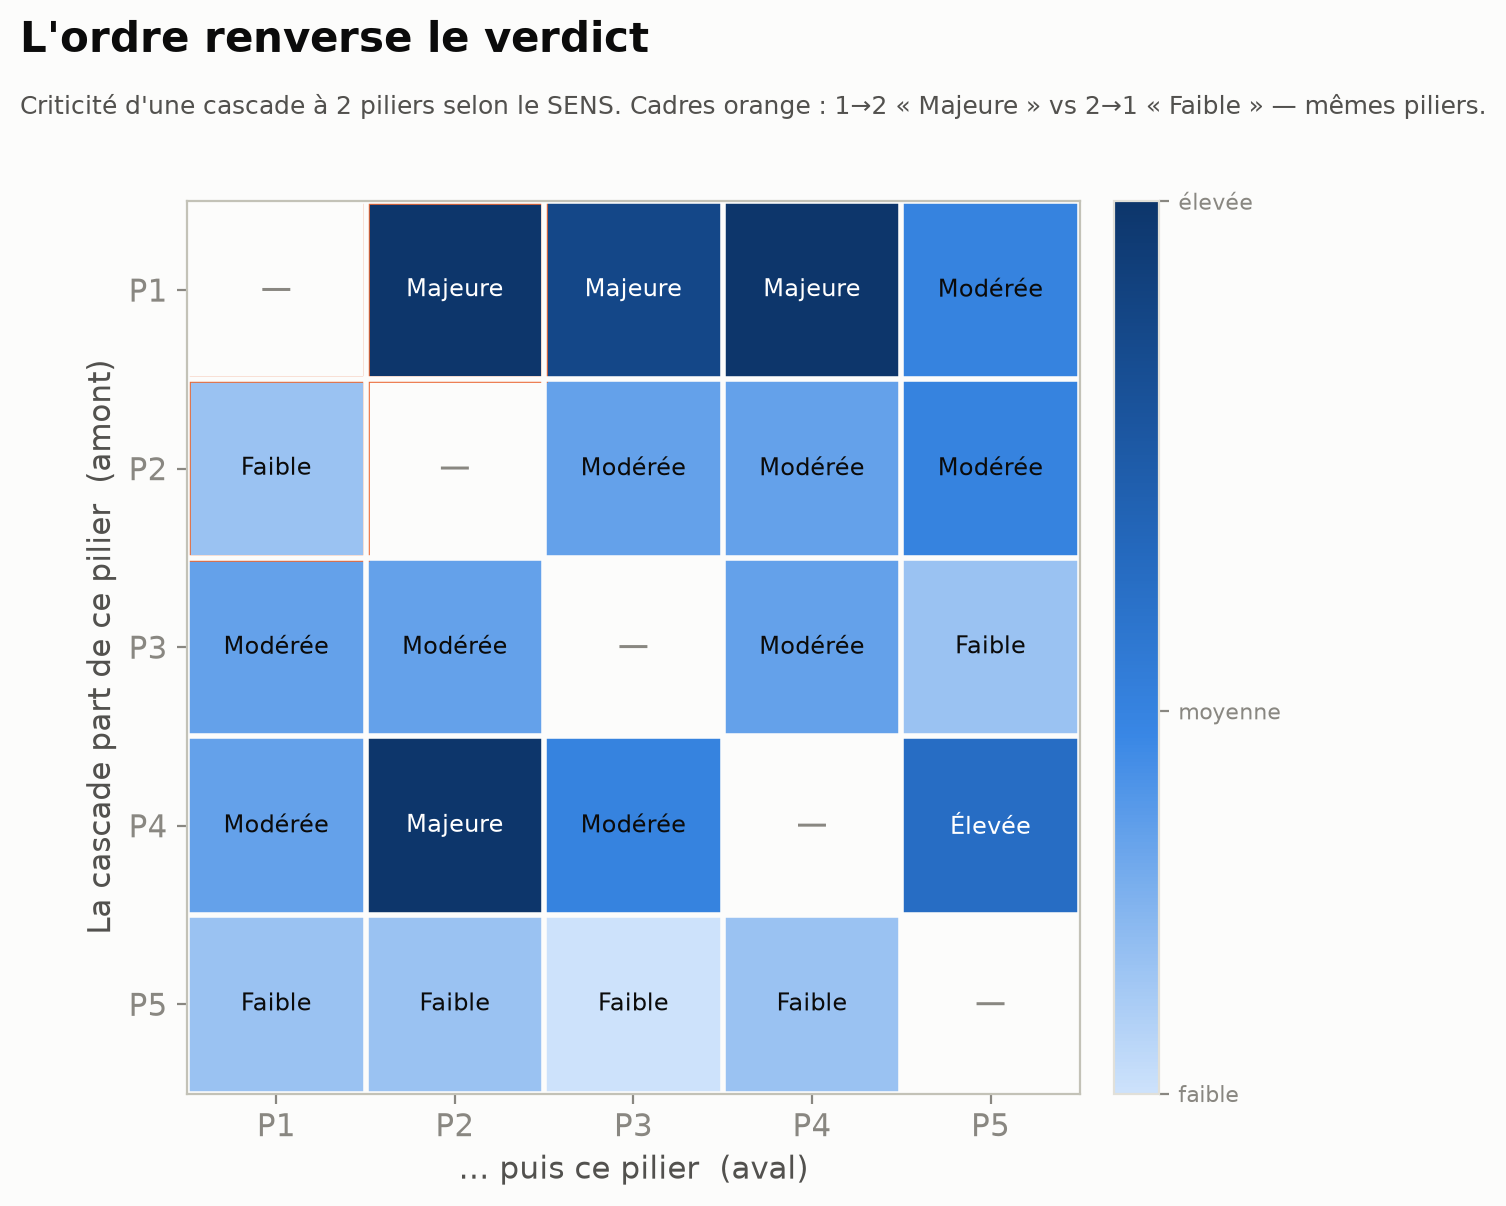
\includegraphics[height=0.70\textheight]{F1_asymetrie_ordre.png}
\end{center}
Mêmes piliers, sens opposés : 1 vers 2 ressort \textbf{Majeure}, 2 vers 1 ressort
\textbf{Faible}. Une simple corrélation serait symétrique et raterait cela.
\end{frame}

% =====================================================================
\begin{frame}{Le pilier qui amorce fait le verdict}
\begin{center}
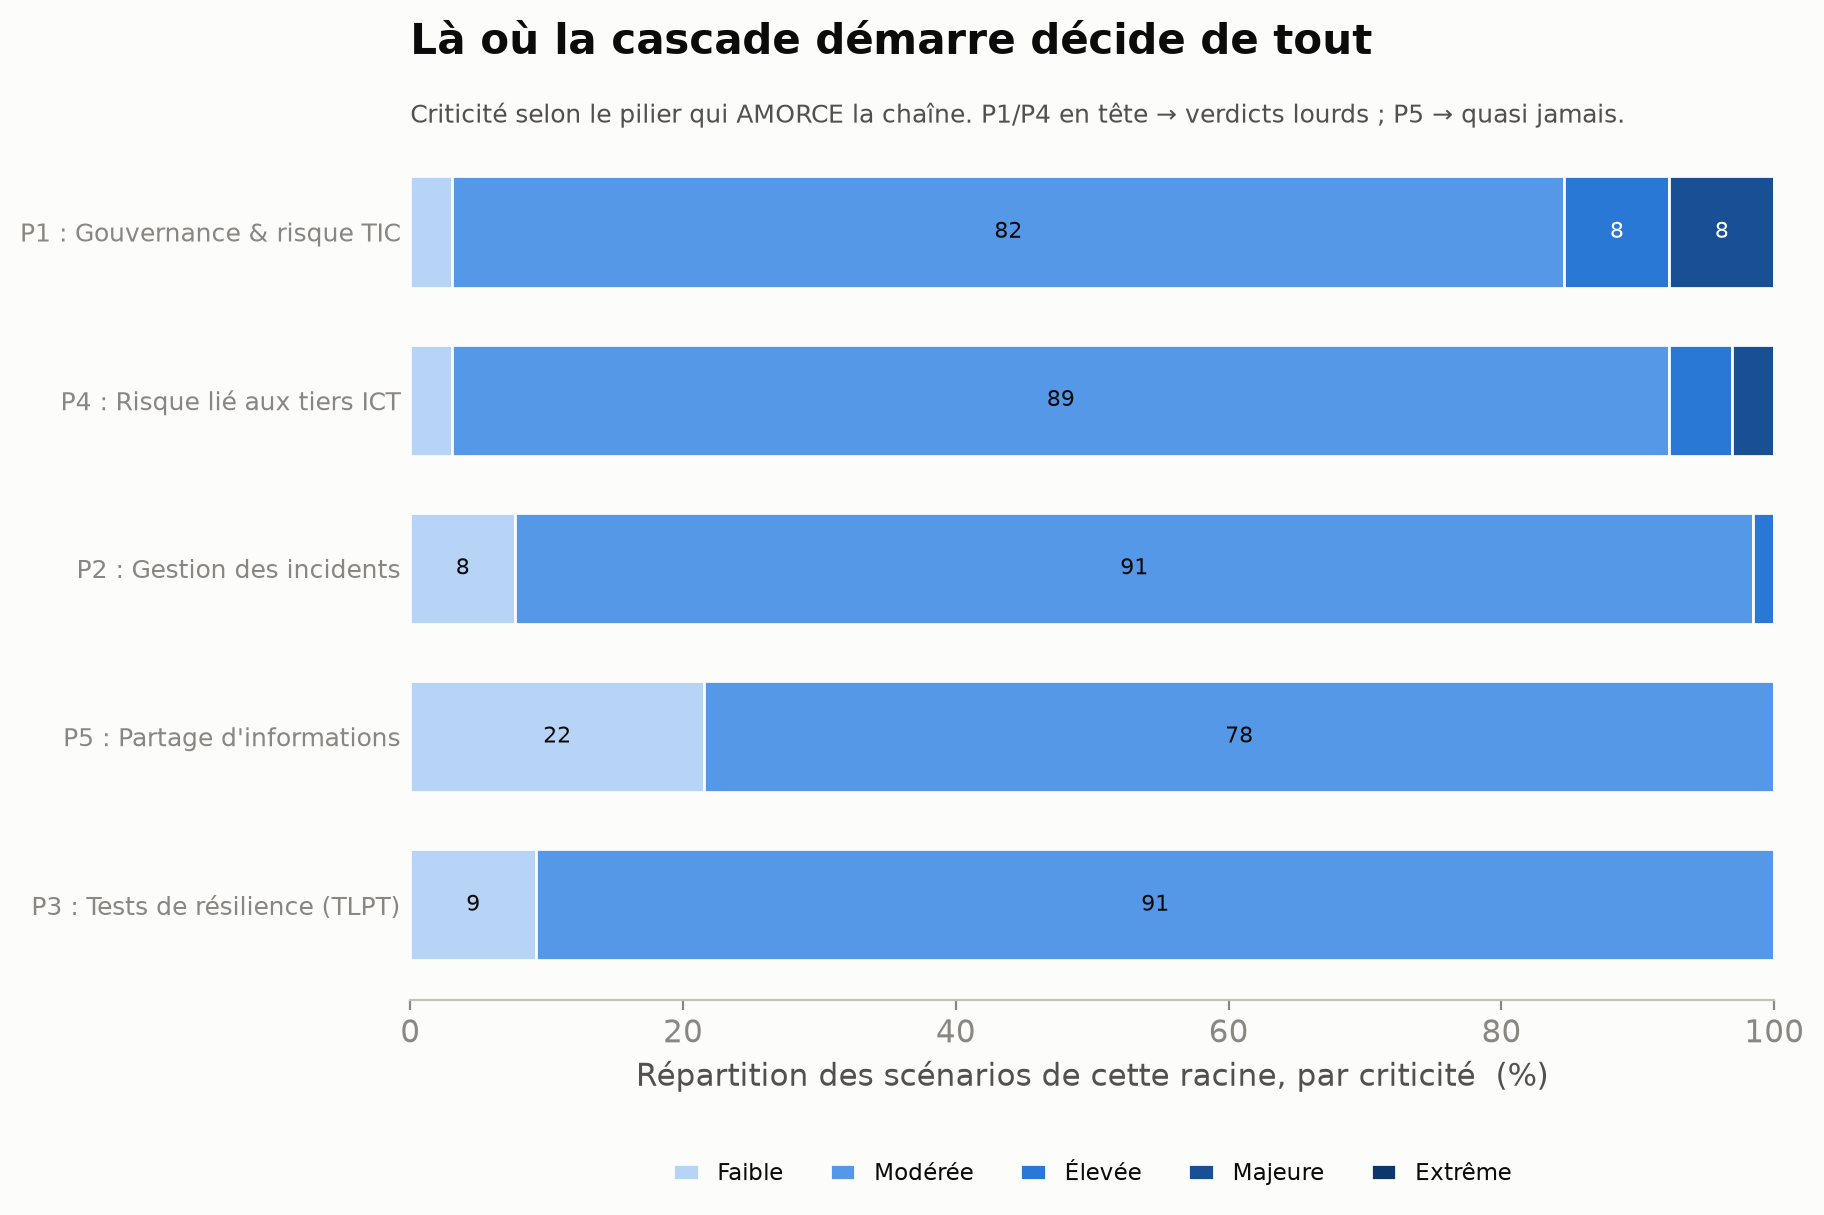
\includegraphics[width=0.96\linewidth]{F5_pilier_racine.png}
\end{center}
Une cascade amorcée par \textbf{P1} ou \textbf{P4} donne des verdicts lourds ;
amorcée par \textbf{P5}, presque jamais.
\end{frame}

% =====================================================================
\begin{frame}{Les scénarios les plus critiques}
\begin{center}
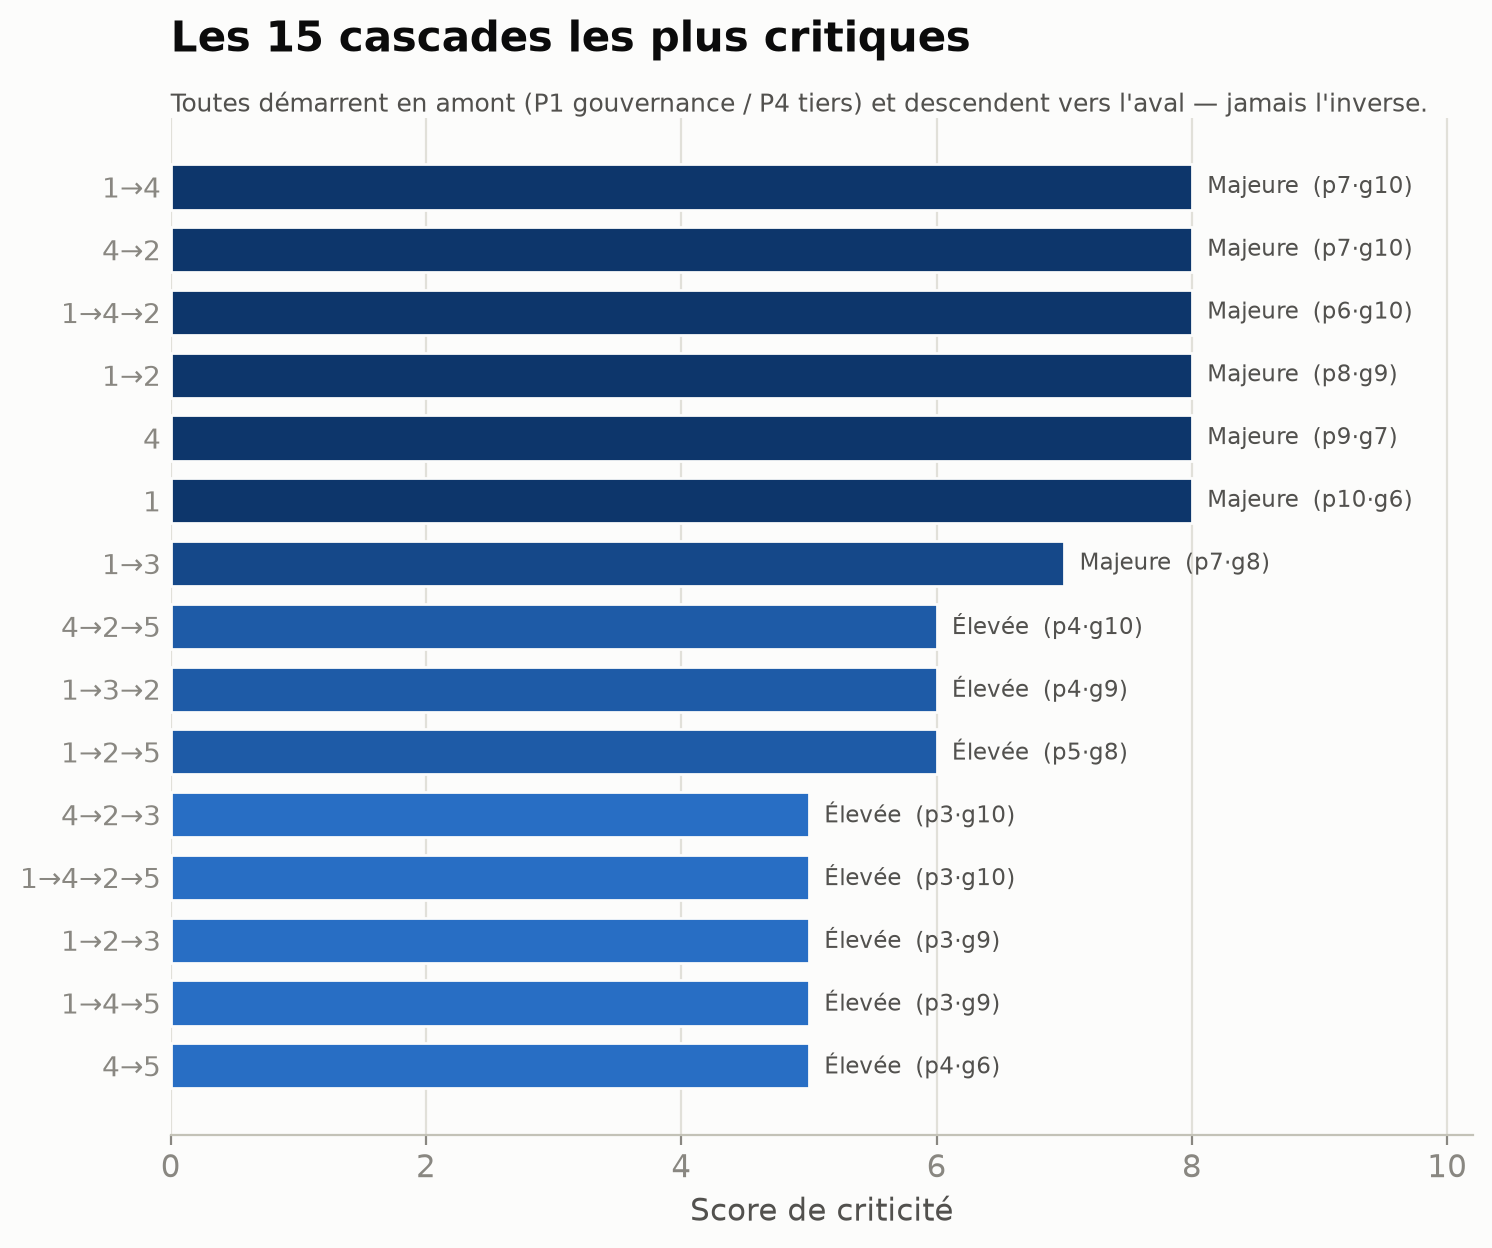
\includegraphics[height=0.70\textheight]{F4_top_cascades.png}
\end{center}
En tête : des cascades qui partent de l'amont (gouvernance, tiers) vers l'aval, jamais
l'inverse. Les scores ne servent qu'à trier ; on lit des catégories.
\end{frame}

% =====================================================================
\begin{frame}{Du classement au capital : la contagion}
Jusqu'ici c'est \textbf{qualitatif}. Pour le capital, on injecte la même information
d'expert (le \og{}qui entraîne qui\fg{}) dans le modèle quantitatif.
\begin{itemize}
\item Un pilier sous stress \textbf{contamine} les autres piliers de la même entité :
      une \textbf{boucle de contagion}, pas une corrélation posée après coup.
\item On \textbf{borne} cette boucle pour qu'elle reste stable (sinon la perte part à
      l'infini).
\end{itemize}
\vfill
\begin{block}{Honnêteté sur le statut}
C'est une adaptation d'un modèle de risque de crédit (Vasicek) : on gagne la contagion
dirigée, au prix de certaines propriétés théoriques. On l'assume et on le dit.
\end{block}
\end{frame}

% =====================================================================
\begin{frame}{Une cascade doit pouvoir s'éteindre}
\begin{itemize}
\item Sans garde-fou, la chaîne ne s'arrête jamais et la sévérité explose.
\item On donne à chaque pilier une \textbf{probabilité de tout arrêter}.
\item \textbf{P5} (partage d'informations) éteint souvent la cascade ; \textbf{P1} presque
      jamais.
\item Règle : un pilier ne défaille qu'une fois (cascade \og{}auto-évitante\fg{}).
\end{itemize}
\vfill
Résultat : une perte finie, et des piliers naturellement en bout de chaîne (comme P5).
\end{frame}

% =====================================================================
\begin{frame}{Là où j'ai besoin de ton avis}
\small
\begin{enumerate}
\item \textbf{Calibrer la contagion} (le \og{}qui entraîne qui\fg{}) : aujourd'hui c'est du
      jugement d'expert. Les bases de pertes ne codent pas les piliers \textbf{co-touchés},
      les bases de brèches n'ont pas l'\textbf{horodatage} fin.
      \begin{itemize}\small
      \item Existe-t-il, chez tes clients ou en interne, un \textbf{registre d'incidents
            horodaté} (proche du format de reporting DORA) exploitable ? Sur quel périmètre ?
      \end{itemize}
\item \textbf{La sévérité} : aujourd'hui la gravité d'un pilier est un \textbf{score
      ordinal}, pas un montant. Comment passer proprement à des \textbf{euros par pilier} ?
\item \textbf{Le réalisme de terrain} : l'ordre P1/P4 en amont, P5 en aval, ça colle à ce
      que tu vois en mission ?
\end{enumerate}
\end{frame}

% =====================================================================
\begin{frame}{Ce que je retiens de cet échange}
\begin{itemize}
\item Ta lecture opérationnelle de l'ordre des piliers (amont vers aval).
\item Une piste de \textbf{donnée} : incidents codés par pilier et/ou horodatés.
\item Une \textbf{maille de coût} par pilier crédible côté métier.
\end{itemize}
\vfill
\begin{center}
Merci. Je te laisse les slides et les PDF détaillés pour ton retour.
\end{center}
\end{frame}

\end{document}
